\documentclass[../sparc.tex]{subfiles}
\graphicspath{{\subfix{../images/}}}
\begin{document}

%%%%%%%%%%%%%%%%%%%%%%%%%%%%%%%%%%%%%%%%%%%%%%%%%%%%%%%%%%%%%%%%%%%%%%%%%%%%%%%%
\section{Resistance}
\label{section:electronics-resistance}
\index{Electronics!Resistance}

To be able to calculate the speed of the water flowing from one vessel to
another we have to know the parameters of the pipe that connecting the vessels --
in the other words, the parameters of the \emph{water conductor}.  And one of
the main parameter is the \emph{resistance} of the pipe.  The greater the
resistance, the slower the water will flow.

We can use a pipe with a small inner diameter as an example of water conductor
with high resistance, as shown on fig. \ref{fig:electronics-resistance-0}.

\begin{figure}[ht]
  \centering
  \def\offset{6}
  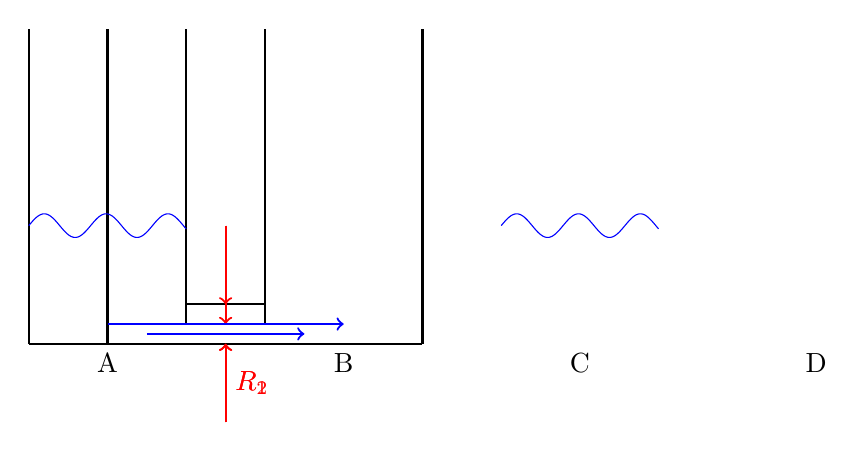
\begin{tikzpicture}[
      declare function={f1(\x) = 0.15 * sin(8.0 * deg(\x));
    }]

    \draw[thick] (0, 0) -- (0, 4);
    \draw[thick] (2, 0.5) -- (2, 4);
    \draw[thick] (0, 0) -- (2, 0);

    \draw[thick] (3, 0.5) -- (3, 4);
    \draw[thick] (5, 0) -- (5, 4);
    \draw[thick] (3, 0) -- (5, 0);

    \draw[thick] (2, 0) -- (3, 0);
    \draw[thick] (2, 0.5) -- (3, 0.5);

    \draw[thick] (\offset, 0) -- (\offset, 4);
    \draw[thick] (\offset + 2, 0.25) -- (\offset + 2, 4);
    \draw[thick] (\offset, 0) -- (\offset + 2, 0);

    \draw[thick] (\offset + 3, 0.25) -- (\offset + 3, 4);
    \draw[thick] (\offset + 5, 0) -- (\offset + 5, 4);
    \draw[thick] (\offset + 3, 0) -- (\offset + 5, 0);

    \draw[thick] (\offset + 2, 0) -- (\offset + 3, 0);
    \draw[thick] (\offset + 2, 0.25) -- (\offset + 3, 0.25);

    \draw[thick, color=red, ->] (2.5, 1.5) -- (2.5, 0.5);
    \draw[thick, color=red, ->] (2.5, -1) -- (2.5, 0);
    \draw[color=red] (2.5, -0.5) node[right] {$R_1$};

    \draw[thick, color=red, ->] (\offset + 2.5, 1.5) -- (\offset + 2.5, 0.25);
    \draw[thick, color=red, ->] (\offset + 2.5, -1) -- (\offset + 2.5, 0);
    \draw[color=red] (\offset + 2.5, -0.5) node[right] {$R_2$};

    \draw[thick, color=blue, ->] (1, 0.25) -- (4, 0.25);

    \draw[thick, color=blue, ->] (\offset + 1.5, 0.125) -- (\offset + 3.5, 0.125);

    \begin{scope}[yshift=1.5cm, color=blue]
      \draw (0, 0) plot[domain=0:2, variable=\x, samples=200, smooth] ({\x}, {f1(\x)});
    \end{scope}

    \begin{scope}[yshift=1.5cm, xshift=6 cm, color=blue]
      \draw (0, 0) plot[domain=0:2, variable=\x, samples=200, smooth] ({\x}, {f1(\x)});
    \end{scope}

    \draw (1, 0) node[below] {A};
    \draw (4, 0) node[below] {B};
    \draw (7, 0) node[below] {C};
    \draw (10, 0) node[below] {D};

  \end{tikzpicture}
  \caption{An example of two vessels connected with pipes with different
    resistance to the water flow.}
  \label{fig:electronics-resistance-0}
\end{figure}

The smaller the inner diameter of a pipe, the higher the resistance.  The same
rule can be applied to an electric conductor (e.g. a piece of wire) where the
diameter of a wire and its resistance have inverse relationship: the thicker the
wire the lesser its resistance to the electric current.  Thus the lesser the
resistance the greater the electric current.

Let's assume that the vessel ``B'' and the vessel ``C'' on
fig. \ref{fig:electronics-resistance-0} are connected with a pipe with one-half
of the pipe diameter that connects vessels ``A'' and ``B''.  Then the water
current between vessels ``B'' and ``C'' will be two times smaller than the water
current between vessels ``A'' and ``B''.

In the electronics we measure the resistance of a conductor in Ohms.

The relationship between current, voltage and resistance is described in
\emph{Ohms Law}.  Using this law we can calculate the electric current for an
electric circuit, using formulae \ref{equation:elemctronics-ohms-law-0}.

\begin{equation}
  \mbox{I} = \frac{\mbox{U}}{\mbox{R}}
  \label{equation:elemctronics-ohms-law-0}
\end{equation}

Where ``I'' is the current (in Amperes), ``U'' is the voltage (in Volts) and
``R'' is resistance (in Ohms.)

In day-to-day life we can be pretty sure that any wire or a piece of some
conducting material (e.g. metal) has some non-zero resistance.  Some materials
have greater resistance than the others.  Such materials that have low
resistance called \emph{conductors}.  Copper, silver and gold are examples of
good conductors.  Materials that have high resistance commonly used as
\emph{insulator} and they are called \emph{dielectric}.  We can put in this
category different kinds of plastics that are used as the material for wire
insulators.

\experiment{0}{Look around you -- how many conductors can you find?}

When electric current flows through a conductor that has some resistance (that
is, through any common conductive material) some percentage of the energy get
lost by turning into heat radiated from the conductor.  For example when you
plug an electric kettle into a power socket and turn it on, not only the kettle
heater gets hot, but the wires that conduct the electricity from the wall socket
to the kettle.  Although the heating of wires is miniscule in comparison the the
temperature of the water heater inside the kettle.

In some cases the heating of a conductor is the desired effect itself as in the
case of an electric kettle; in other cases engineers try to lower the resistance
of a conductor that in turn lower the heating -- because the heating is but an
energy loss and is unwanted.

\experiment{1}{Can you name other examples where the heating of a conductor is
  desired?}

There are conductors that don't have resistance -- they called
\emph{super-conductors}.  Nowadays this type of conductors can be found only in
specific devices (such as scientific equipment) where it is required to conduct
electric current without energy loss due to heat.  In everyday life application
of super-conductors is problematic due to their high price and exotic
requirements for operating conditions (for example, modern super-conductors
require very low temperature for the super-conducting effects to occur.)

Not only most of conductors have resistance, but voltage source have their own
resistance as well -- it is called \emph{internal resistance of the voltage
source}.

In electronics resistance with the required value and error percentage is set by
a special electronic component called \emph{resistor}.

Resistors play important role in electric circuits as they allow to control the
electric current in the circuit.  As every electronic component have specific
operating conditions it is important to pass the electric current limited by the
borders set for the specific component.  Thus if we connect a resistor with the
resistance value calculated from the specifications of LED we will protect the
LED from the premature failure.  The schematic is shown on
fig. \ref{fig:electronics-circuit-resistors}.

\begin{figure}[ht]
  \centering
  \begin{circuitikz}
    \draw
    (0, 0) to[battery, l=Battery]
    (0, 4) to[short]
    (1, 4) to[resistor, l=$R_1$] (3, 4)
    (3, 4) to[full led, l=LED] (7, 4)
    (7, 4) to[short]
    (7, 0) to[short]
    (0, 0);
  \end{circuitikz}
  \caption{An electric circuit with an LED and a $R_1$ resistor that limits the
    current.}
  \label{fig:electronics-circuit-resistors}
\end{figure}

\index{Electronics!Resistance!Serial Resistor Connection}

When resistors are connected in a serial manner their resistance values are
added.  To draw an analogy with water we can say that when we make a pipe longer
its resistance to the water flow becomes higher.
Fig. \ref{fig:electronics-resistance-1} shows two vessels connected with a
pipeline made by two pipes joined together in sequence; the resistance of the
resulting pipeline to the water flow between vessel ``A'' and vessel ``B'' is
equal to the sum of the resistance $R_1$ and $R_2$.  Thus the total resistance
of the pipeline is greater than $R_1$ and $R_2$ on its own.

\begin{figure}[ht]
  \centering
  \def\offset{0}
  \begin{tikzpicture}[
      declare function={f1(\x) = 0.15 * sin(8.0 * deg(\x));
    }]

    \draw[thick] (\offset, 0) -- (\offset, 4);
    \draw[thick] (\offset + 2, 0.5) -- (\offset + 2, 4);

    \draw[thick] (\offset + 4, 0.25) -- (\offset + 4, 4);
    \draw[thick] (\offset + 6, 0) -- (\offset + 6, 4);

    %% "Труба" между ёмкостями "В" и "Г".
    \draw[thick] (\offset, 0) -- (\offset + 6, 0);
    \draw[thick] (\offset + 2, 0.5) -- (\offset + 3, 0.5);
    \draw[thick] (\offset + 3, 0.5) -- (\offset + 3, 0.25);
    \draw[thick] (\offset + 3, 0.25) -- (\offset + 4, 0.25);

    \draw[thick, color=blue, ->] (\offset + 1, 0.125) -- (\offset + 5, 0.125);

    \draw[thick, color=red, <->] (2, 1) -- (3, 1);
    \draw[color=red] (2.5, 1) node[above] {$R_1$};

    \draw[thick, color=red, <->] (\offset + 2, 1) -- (\offset + 3, 1);
    \draw[color=red] (\offset + 2.5, 1) node[above] {$R_1$};
    \draw[thick, dotted, color=red] (\offset + 3, 2) -- (\offset + 3, -1);
    \draw[thick, color=red, <->] (\offset + 3, 1) -- (\offset + 4, 1);
    \draw[color=red] (\offset + 3.5, 1) node[above] {$R_2$};

    \begin{scope}[yshift=1.5cm, color=blue]
      \draw (0, 0) plot[domain=0:2, variable=\x, samples=200, smooth] ({\x}, {f1(\x)});
    \end{scope}

    \draw (1, 0) node[below] {А};
    \draw (5, 0) node[below] {Б};

  \end{tikzpicture}
  \caption{A sequential connection of resistances with water used as an
    example.}
  \label{fig:electronics-resistance-1}
\end{figure}

The equation \ref{equation:elemctronics-resistance-0} allows to calculate the
total resistance of a conductor in case of sequential connection of resistances.

\begin{equation}
  \mbox{R}_{\mbox{total}} = \mbox{R}_{\mbox{1}} + \mbox{R}_{\mbox{2}}
  \label{equation:elemctronics-resistance-0}
\end{equation}

An example of electric circuit with sequential connection of resistors is shown
on fig. \ref{fig:electronics-circuit-resistors-in-series}.

\begin{figure}[ht]
  \centering
  \begin{circuitikz}
    \draw
    (0, 0) to[battery, l=Battery]
    (0, 4) to[short]
    (1, 4) to[resistor, l=$R_1$] (3, 4)
    (3, 4) to[resistor, l=$R_2$] (5, 4)
    (5, 4) to[full led, l=LED] (7, 4)
    (7, 4) to[short]
    (7, 0) to[short]
    (0, 0);
  \end{circuitikz}
  \caption{Sequential connection of resistors $R_1$ and $R_2$.}
  \label{fig:electronics-circuit-resistors-in-series}
\end{figure}

\index{Electronics!Resistance!Parallel Resistor Connection}

Another way of lower the resistance is to use several conductors connected in
\emph{parallel} as shown on fig. \ref{fig:electronics-resistance-2}.

\begin{figure}[ht]
  \centering
  \def\offset{6}
  \begin{tikzpicture}[
      declare function={f1(\x) = 0.15 * sin(8.0 * deg(\x));
    }]

    \draw[thick] (0, 0) -- (0, 4);
    \draw[thick] (2, 0.5) -- (2, 1);
    \draw[thick] (2, 1.5) -- (2, 4);
    \draw[thick] (0, 0) -- (2, 0);

    \draw[thick] (3, 0.5) -- (3, 1);
    \draw[thick] (3, 1.5) -- (3, 4);
    \draw[thick] (5, 0) -- (5, 4);
    \draw[thick] (3, 0) -- (5, 0);

    \draw[thick] (2, 0) -- (3, 0);
    \draw[thick] (2, 1.5) -- (3, 1.5);
    \draw[thick] (2, 1.0) -- (3, 1.0);
    \draw[thick] (2, 0.5) -- (3, 0.5);

    \draw[thick, color=blue, ->] (1, 1.25) -- (4, 1.25);
    \draw (3.5, 1.25) node[above, color=red] {$R_1$};
    \draw[thick, color=blue, ->] (1, 0.25) -- (4, 0.25);
    \draw (3.5, 0.25) node[above, color=red] {$R_2$};

    \begin{scope}[yshift=3cm, color=blue]
      \draw (0, 0) plot[domain=0:2, variable=\x, samples=200, smooth] ({\x}, {f1(\x)});
    \end{scope}

    \draw (1, 0) node[below] {А};
    \draw (4, 0) node[below] {Б};
  \end{tikzpicture}
  \caption{An example of two vessels connected with a pipeline consisting of two
    pipes that run in parallel.}
  \label{fig:electronics-resistance-2}
\end{figure}

In this case the total resistance of the pipeline is less than the lesser
resistance in the pipe group.

An equation to calculate the total resistance for two parallel connections in a
circuit is shown in \ref{equation:elemctronics-resistance-1}.

\begin{equation}
  \mbox{R}_{\mbox{total}} = \frac{\mbox{R}_{\mbox{1}} * \mbox{R}_{\mbox{2}}}{\mbox{R}_{\mbox{1}} + \mbox{R}_{\mbox{2}}}
  \label{equation:elemctronics-resistance-1}
\end{equation}

This equation allows to calculate the total resistance of any number of
conductors connected in parallel on a segment of a circuit.

An electric circuit with two resistors connected in parallel is shown on fig.
\ref{fig:electronics-circuit-parallel-resistors}.

\begin{figure}[ht]
  \centering
  \begin{circuitikz}
    \draw
    (0, 0) to[battery, l=Battery]
    (0, 4) to[short]
    (1, 4) to[short]
    (1, 5) to[resistor, l=$R_1$] (4, 5) -- (4, 4);
    \draw
    (1, 4) to[short]
    (1, 3) to[resistor, l=$R_2$] (4, 3) -- (4, 4);
    \draw
    (4, 4) to[full led, l=LED] (6, 4)
    (6, 4) to[short]
    (6, 0) to[short]
    (0, 0);
  \end{circuitikz}
  \caption{Parallel connection of resistors $R_1$ and $R_2$.}
  \label{fig:electronics-circuit-parallel-resistors}
\end{figure}


\end{document}
